\documentclass{elsarticle}

\usepackage{amsmath,bm}
\usepackage{algorithm}
\usepackage{algpseudocode}
\usepackage{minted}
\usepackage{xcolor}

\begin{document}

\begin{frontmatter}
\author{Ashwin Srinath}
\title{A fast GPU solver for near-Toeplitz tridiagonal systems}
\maketitle

\begin{abstract}

\end{abstract}

\end{frontmatter}

%----------------------------------------------------------------------%
    
\section{Introduction}

In this paper, we consider the solution of
linear systems of the form $A\bm{x} = \bm{d}$,
where $A$ has the following structure

\begin{equation} \label{eqn:toeplitz-matrix}
A = 
\begin{pmatrix}
     b_1 & c_1  \\
     a_0 & b_0  &  c_0  \\
         & a_0  &  b_0 &  c_0  \\
         &      &  a_0 &  b_0 &  c    \\
         &      &      &      &  \ddots \\
         &      &      &      &     &  \ddots  \\
         &      &      &      &     &  a_n  &  b_n
\end{pmatrix}
\end{equation}

Where, in general
\begin{align*}
    & a_0 \neq a_n & \\
    & b_1 \neq b_0 \neq b_n &\\
    & c_1 \neq c_0 &
\end{align*}

We refer to matrices with the specific structure of $A$
as \emph{near-Toeplitz tridiagonal matrices},
and the linear system $A\bm{x}=\bm{d}$ as \emph{near-Toeplitz tridiagonal systems}.

The solution of such tridiagonal systems
appears in several numerical schemes
in Computational Fluid Dynamics (CFD)
such as
compact finite differences \cite{lele1992compact},
Alternating Direction Implicit (ADI) methods \cite{1955ADI}, and
numerical solutions to one-dimensional differential equations.
In such applications,
the evaluation of the tridiagonal systems constitutes
a significant portion of the runtime.
Recently, there has been considerable interest in the CFD community
in developing general tridiagonal solvers that
exploit the massive parallelism afforded by
Graphics Processing Units (GPUs)
to speed up the computations
\cite{tutkun2012gpu}
\cite{esfahanian2014efficient}
\cite{GoSt11CR}.
The performance of tridiagonal solvers on the GPU
has been shown to depend on several factors,
such as
choice of algorithm and the associated complexity,
thread utilization,
use of the available memory hierarchy,
and synchronization and control costs
\cite{Zhang2010FTS}.
Many approaches described in the literature
seek to make trade-offs between these factors
to arrive at a solver that best fits the requirements.
But to our knowledge,
the algorithms proposed so far
are applicable to general tridiagonal systems,
and make no attempt to take advantage of
the known structure of the tridiagonal matrix.
We describe the implementation of a GPU solver that
uses this information to
reduce the number of computations
and memory accesses.
The resulting solver is thus able to perform twice as fast as
the equivalent NVIDIA CUSPARSE solver,
and an Intel MKL solver running with 16 independent cores.

This paper is organized as follows:
Section \ref{sec:preliminaries}
describes algorithms for solving tridiagonal systems on GPUs.
The cyclic reduction algorithm in particular, is discussed in detail,
and issues with its implementation on GPUs is discussed.
Section \ref{sec:proposed-algorithm}
describes our proposed solver for near-Toeplitz tridiagonal systems.
Section \ref{sec:results-single-gpu}
provides an overview of the performance of our solver,
and compares it with other implementations.

%----------------------------------------------------------------------%
\section{Preliminaries} \label{sec:preliminaries}

\subsection{Cyclic reduction} \label{subsec:cyclic-reduction}

\begin{equation} \label{eqn:general-tridiagonal-system}
\begin{pmatrix}
     b_1 & c_1  \\
     a_2 & b_2  &  c_2  \\
         & a_3  &  b_3 &  c_3  \\
         &      &  a_4 &  b_4 &  c_4  \\
         &      &      &      &  \ddots \\
         &      &      &      &     &  \ddots  \\
         &      &      &      &     &  a_n  &  b_n
\end{pmatrix}
\begin{bmatrix}
    x_1 \\
    x_2 \\
    x_3 \\
    x_4 \\
    \vdots \\
    \vdots \\
    x_n
 \end{bmatrix}
=
\begin{bmatrix}
   d_1 \\
   d_2 \\
   d_3 \\
   d_4 \\
   \vdots \\
   \vdots \\
   d_{n}
\end{bmatrix}
\end{equation}

Cyclic reduction is applicable to the solution of
general linear systems of the form $Ax = d$,
where $A$ is a tridiagonal matrix with diagonals
$a$, $b$ and $c$
(Equation \ref{eqn:general-tridiagonal-system}).
The algorithm consists of two phases:
\emph{forward reduction} and \emph{backward substitution}.
In the forward reduction phase,
every even-indexed equation $i$
is expressed as a
linear combination of equations $i$, $i-1$ and $i+1$,
yielding a new tridiagonal system of
$n/2$ equations in $n/2$ unknowns
(Equations \ref{eqn:forward-reduction-1} - \ref{eqn:forward-reduction-4}).
The process is repeated until a system of
2 equations in 2 unknowns is left.

\begin{align} 
& a^{\prime}_i = -a_{i-1}k_1 \
    \label{eqn:forward-reduction-1}& \\
& b^{\prime}_i = b_i - c_{i-1}k_1 - a_{i+1}k_2 \
    \label{eqn:forward-reduction-2}& \\
& c^{\prime}_i = -c_{i+1}k_2 \
    \label{eqn:forward-reduction-3}& \\
& d^{\prime}_i = d_i - d_{i-1}k_1  - d_{i+1}k_2 \
    \label{eqn:forward-reduction-4}&
\end{align}

where,

\begin{align}
& k_1 = \frac{a_i}{b_{i-1}} \label{eqn:k1-update}& \\
& k_2 = \frac{c_i}{b_{i+1}} \label{eqn:k2-update}&
\end{align}

The 2-by-2 system of equations is solved trivially,
yielding $x_n$ and $x_{n/2}$.
In the backward substitution phase,
every odd-indexed unknown $x_i$ is solved for by
substituting the known values of $x_{i-1}$ and $x_{i+1}$
(Equation \ref{eqn:backward-substitution}) .

\begin{align} \label{eqn:backward-substitution}
x_i = \frac{d^{\prime}_i - a^{\prime}_ix_{i-1} - \
    c^{\prime}_ix_{i+1}}{b^{\prime}_i}
\end{align}

For the last index $i=n$,
the forward reduction step is instead:
\begin{align} \label{eqn:forward-reduction-last}
    & a^{\prime}_n = -a_{n-1}k_1 & \\
    & b^{\prime}_n = b_n - c_{n-1}k_1 & \\
    & d^{\prime}_n = d_n - d_{n-1}k_1&
\end{align}

And for $i=1$, the backward substitution step is instead:
\begin{align} \label{eqn:backward-substitution-first}
x_1 = \frac{d^{\prime}_1 - c^{\prime}_1x_{2}}{b^{\prime}_1}
\end{align}

Thus, in the best case ($n$ parallel processors),
cyclic reduction requires 
$2log(n) - 1$ steps.
For even moderately large $n$,
this is significantly smaller than
the $2n$ steps required by the classical Thomas algorithm.
This makes cyclic reduction a good fit
for massively parallel architectures like GPUs.

\begin{figure}[h!]
\begin{center}
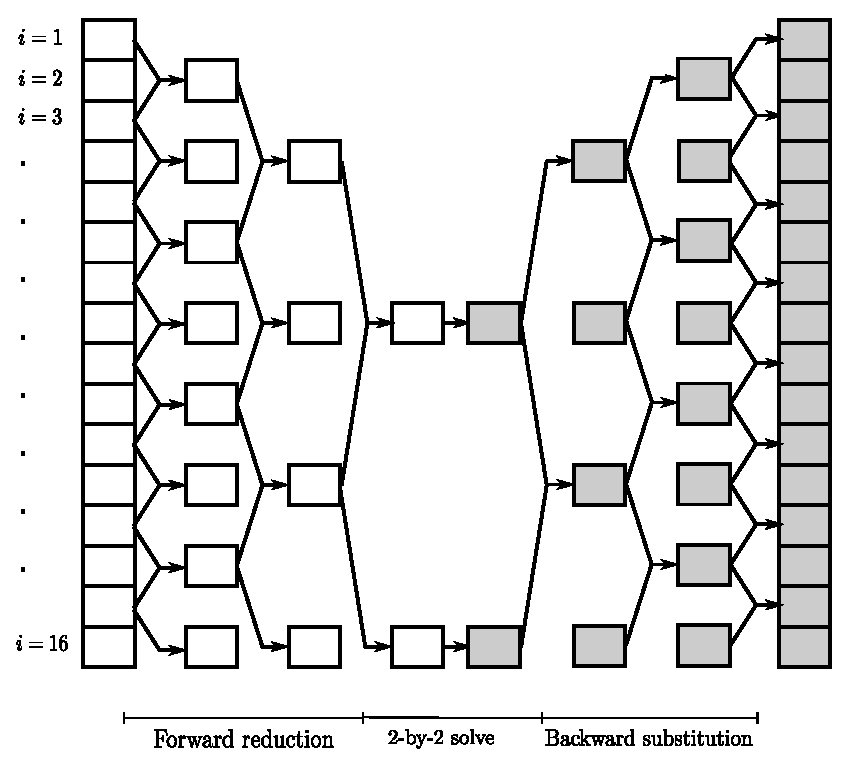
\includegraphics[height=250pt]{img/cyclic-reduction.eps}
\end{center}
\caption{Cyclic reduction}
\label{fig:cyclic-reduction}
\end{figure}

\subsection{GPU architecture} \label{subsec:gpu-architecture}

Writing applications that effectively exploit the GPU
requires a thorough understanding of the underlying architecture.
We provide the pertinent details here,
and refer to \cite{GPUcomputingera} for a more complete picture.
Our tests are performed on the NVIDIA Tesla K20 and K40 GPUs,
built on the ``Kepler'' architecture,
an overview of which is available at \cite{Keplerwhitepaper}.

Applications that use the GPU include special
pieces of code that are executed on the GPU,
referred to as \emph{kernels}.
In C, for example, kernels are written as functions,
and are called with (almost) the same conventions.
A kernel is executed in parallel by several lightweight threads,
which are organized into a \emph{grid} of \emph{thread blocks}
(or just \emph{blocks}).
As a requirement, thread blocks must be able to run
independent of each other,
in series or in parallel.

From the hardware perspective, an NVIDIA GPU may be viewed primarily as
a collection of so-called Streaming Microprocessors (SMs).
When a kernel is launched (with a specified number of thread blocks),
each block is assigned to an SM.
Threads within a thread block can execute concurrently on the SM,
and an SM can execute several thread blocks concurrently.
The number of thread blocks that an SM can execute concurrently
is limited by a number of factors,
and maximizing this number is often key to obtaining good performance.

Every thread in every block has access to so-called \emph{global memory},
which can also be accessed by the CPU (or \emph{host}) via the PCI-e bus.
Further,
threads within a thread block have access
to a common, fast, limited \emph{shared memory}.
The contents of shared memory are managed by the kernel code,
and shared memory is often viewed as an explicitly controlled cache.
Each thread also has private \emph{local memory},
and access to extremely fast registers.
Unlike CPUs, the GPU has a large number of registers---a
thread executing a kernel will
typically attempt to store the variables defined in registers,
before spilling over to local memory, which is much slower.

Thread access to global memory is slow,
and is especially inefficient when
successive threads in a block
access locations that are far apart in memory---known
as \emph{uncoalesced} memory access.
Shared memory access can be expected to be
much faster than global memory---however,
the amount of shared memory per SM is limited
(48 KiB for current GPUs).
The amount of shared memory actually used by each block,
can thus limit the number of blocks that
concurrently run on each SM---known as the \emph{occupancy}.
The number of registers per SM is also limited,
and the use of registers can similarly affect occupancy.
Finally, memory transfers between the CPU (host) and GPU (device)
are extremely expensive, limited by the bandwidth of the PCI-e bus.

\subsection{Cyclic reduction implementation on GPU}

\begin{figure}[h!]
\begin{center}
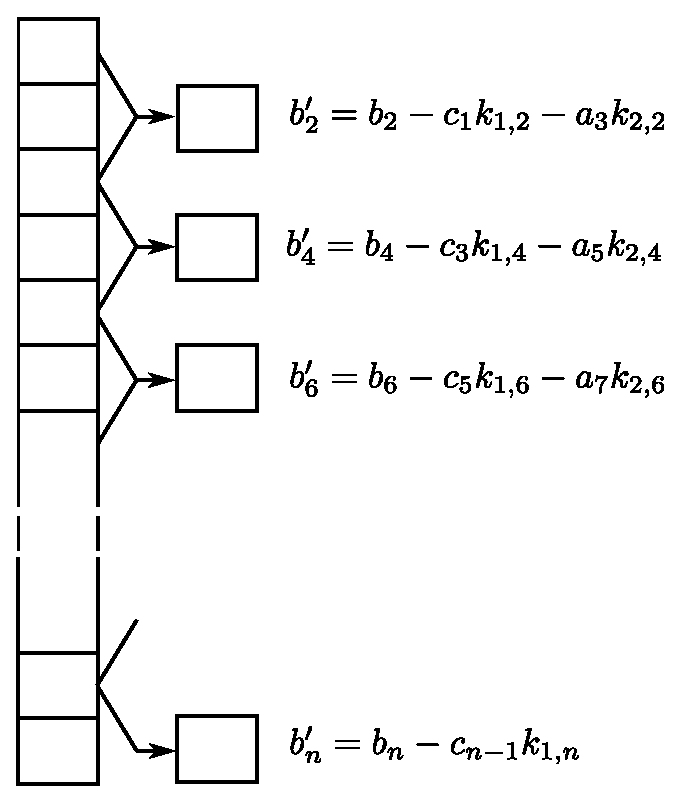
\includegraphics[height=200pt]{img/forward-reduction-step.eps}
\end{center}
\caption{Updating $\bm{b}$ in the first forward reduction step}
\label{fig:forward-reduction-step}
\end{figure}

As described in Section \ref{subsec:gpu-architecture},
GPU instructions are executed concurrently
by several threads and
threads are organized into thread blocks.
In most GPU implementations of cyclic reduction,
blocks are assigned to tridiagonal systems
(when solving multiple systems),
and threads within a block 
are assigned to equations, or \emph{indices}.
(Figure \ref{fig:gpu-mapping})
During the forward reduction phase,
the threads assigned to each even index $i$
compute the coefficients
$a_i^\prime$, $b_i^\prime$ and $c_i^\prime$.
In practice, the coefficients are updated \emph{in-place}
(Figure \ref{fig:forward-reduction-step} shows the updates
to the coefficient array $\bm{b}$ in the first forward reduction step).

In each step of forward reduction,
a thread accesses values from the coefficient arrays
$\bm{a}$, $\bm{b}$ and $\bm{c}$ in a \emph{strided} fashion.
At every subsequent step,
this stride is doubled, while the number of active threads is halved.
In the backward substitution phase,
the strides are halved at each step,
while the number of active threads is doubled.
The long-strided memory accesses towards the end
of the forward reduction
and the beginning of backward substitution
motivates the use of shared memory---strided global memory access is,
in general, associated with performance penalties.
But the limited amount of shared memory places restrictions
on the size of tridiagonal systems that can be solved.
Further,
the memory access pattern in
cyclic reduction leads to \emph{bank conflicts}
\cite{Zhang2010FTS}.
Zhang et al. \cite{Zhang2010FTS} propose a
\emph{hybrid} solver
that uses both cyclic reduction and parallel cyclic reduction
to reduce bank conflicts.
G{\"o}dekke et al. \cite{GoSt11CR}
use a method of separately storing
the even and odd indexed equations
to arrive at a bank-conflict free solver
at the cost of additional shared memory usage.
Shared memory usage is also associated with
lowered GPU occupancy (Section \ref{subsec:gpu-architecture}).
Davidson et al. \cite{davidson2011register}
describe the method of
\emph{register packing}---performing more computations
on \emph{registers}, rather than shared memory---as
a means to reduce shared memory usage in cyclic reduction.
More recently, Esfahanian et al. \cite{esfahanian2014efficient}
describe an implementation of cyclic reduction
that works entirely in global memory,
using additional kernels to reorder data so as to
coalesce memory access.



%----------------------------------------------------------------------%
\section{Proposed algorithm} \label{sec:proposed-algorithm}

\begin{figure}[h!]
\begin{center}
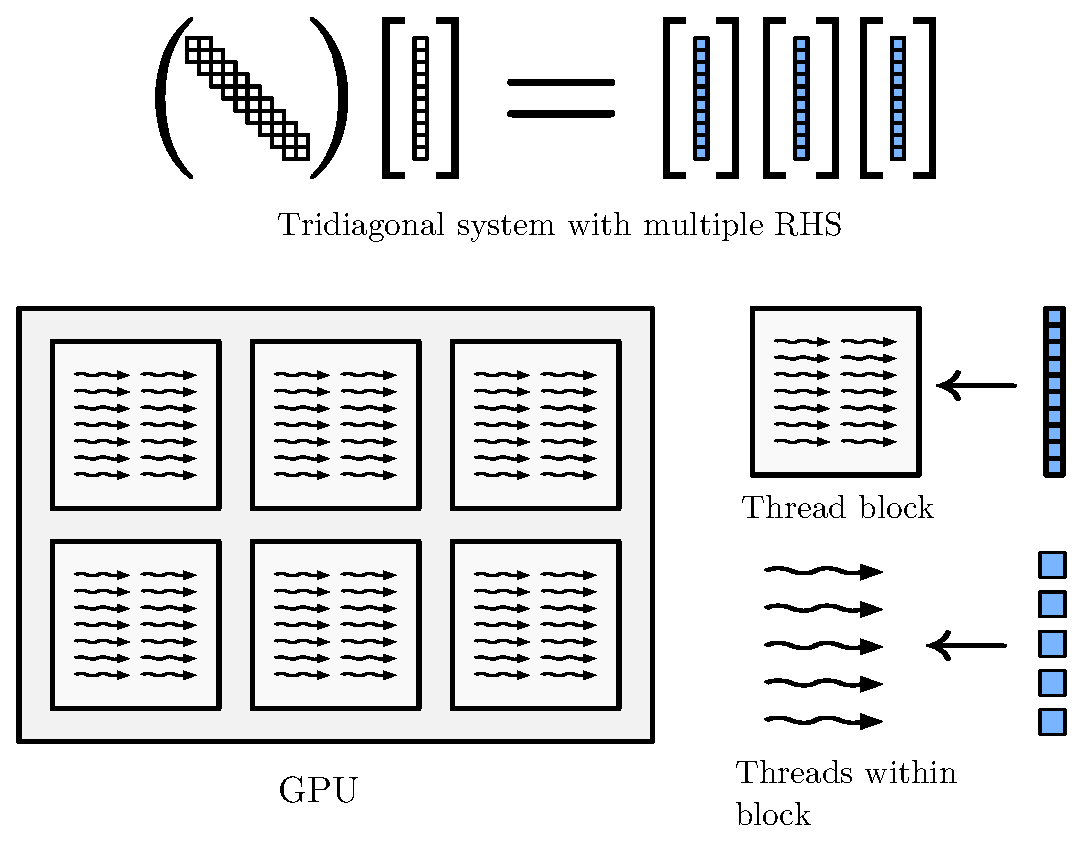
\includegraphics[height=200pt]{img/gpu-mapping.eps}
\end{center}
\label{fig:gpu-mapping}
\caption{Mapping work to blocks and threads:
systems are mapped to blocks and
indices are mapped to individual threads}
\end{figure}

The method is based on precomputing elements 
appearing in the forward reduction phase
so that they can be reused for multiple right hand sides.
While this can be done for general tridiagonal systems,
the applicability to near-Toeplitz systems is
of particular interest due to the lower storage costs.
In Figure \ref{fig:forward-reduction-step},
we list the updates to
$b_i$, for $i=2, 4, 6 ... n$
during the first forward reduction step
for a general tridiagonal matrix.
Similar equations can be written describing
the updates to $a_i$ and  $c_i$.

When the matrix $A$ is near-Toeplitz tridiagonal,
if we substitute in these equations:

\begin{itemize}
    \item [] $a_2 = a_3 = a_4 = \hdots \equiv a_0$
    \item [] $b_2 = b_3 = b_4 = \hdots \equiv b_0$
    \item [] $c_2 = c_3 = c_4 = \hdots \equiv c_0$
\end{itemize}

we observe that the resulting coefficients
$a_i^\prime$, $b_i^\prime$ and $c_i^\prime$
correspond to the coefficients of a tridiagonal matrix with
exactly the near-Toeplitz structure of $A$.
This form-preserving property of cyclic reduction
has been reported for block Toeplitz tridiagonal systems
by Bini et al.

At each reduction step,
for every index $i$,
the coefficients $a_i^\prime$, $b_i^\prime$, $c_i^\prime$
and auxiliary variables $k_1$ and $k_2$
(hereby denoted as $k_{1,i}$ and $k_{2,i}$) are identical,
except for those influenced by the
boundary coefficients of the previous step.
It is possible to \emph{precompute} these values
and store them in separate arrays.
In Figure \ref{fig:cyclic-reduction-precomputing},
it is seen that the space required for storing each of the
forward reduction coefficients
$a_i^\prime$, $b_i^\prime$, $c_i^\prime$,
$k_{1,i}$ and $k_{2,i}$
for a near-Toeplitz matrix
is, at most, $log_2n-2 + 2(log_2n-1)$.

\begin{figure}[h!]
\begin{center}
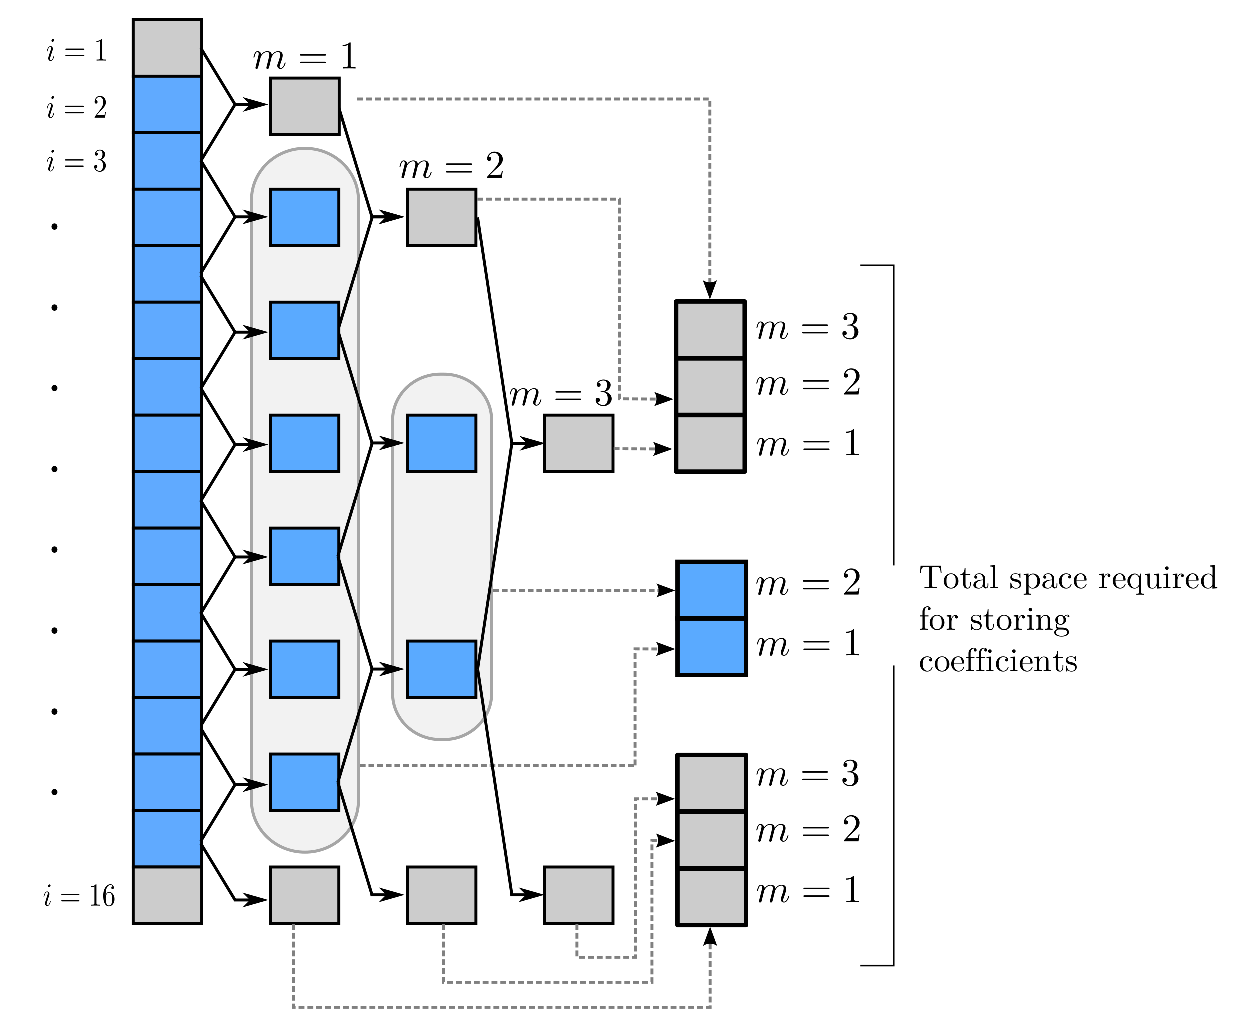
\includegraphics[height=300pt]{img/cyclic-reduction-precomputing.eps}
\end{center}
\caption{Storing forward reduction coefficients
    from each reduction step $m$}
\label{fig:cyclic-reduction-precomputing}
\end{figure}

By precomputing and storing the forward reduction
coefficients,
the $m^{th}$ forward reduction step is reduced to:

\begin{equation}
d^{\prime}_i = d_i - d_{i-1}k_1^{m}  - d_{i+1}k_2^{m}
\label{eqn:precomputed-forward-reduction-step}
\end{equation}

And the $m^{th}$ backward substitution step is:

\begin{equation}
x_i = \frac{d^{\prime}_i - a^mx_{i-1} - \
    c^{m}x_{i+1}}{b^m}
\label{eqn:precomputed-backward-substitution-step}
\end{equation}

Where $a^m$, $b^m$, $c^m$, $k_1^m$ and $k_2^m$
are the appropriate values
from the precomputed coefficient arrays.

\section{GPU implementation} \label{sec:gpu-implementation}

In this section, we describe the implementation of a GPU solver
for solving a given near-Toeplitz tridiagonal system
for $N_{rhs}$ right hand sides.

We describe two approaches based on the common idea
of precomputed forward reduction coefficients---one that leverages
the GPU's \emph{shared memory},
and the other working directly with global memory.
In both approaches,
we map each of the $N_{rhs}$ tridiagonal systems
to blocks,
and equations or \emph{indices} of a system
to individual threads within a block.

Following the algorithm described in \ref{sec:proposed-algorithm},
the forward reduction coefficients
are first computed and loaded into global memory.
The right hand sides are stored in a single
contiguous region global memory.

\subsubsection*{Global memory}

In the global memory approach,
we perform several kernel launches
one for each single forward reduction step,
and another for each backward substitution step.
The precomputed coefficient arrays and right hand
are accessed by the kernels from global memory directly.
Because the coefficients
$k_{1,i}$ and $k_{2,i}$
required in the forward reduction step
(Equation \ref{eqn:precomputed-forward-reduction-step})
are precomputed and available in global memory,
we do not compute
$a_i^\prime$, $b_i^\prime$, $c_i^\prime$,
$k_{1,i}$ and $k_{2,i}$.
This reduces the number of uncoalesced accesses to global memory.
In the backward substitution steps
(Equation \ref{eqn:precomputed-backward-substitution-step}),
the coefficients $a^m$, $b^m$ and $c^m$
are accessed from global memory without coalescing problems.

The advantage of the global memory approach is that
very large tridiagonal systems can be solved without
being limited by the available shared memory per block.
Further,
because we launch a kernel for each
forward reduction and back substitution step,
we can specify the number of threads per block at each launch so that
there are no idle threads throughout the solution process.
($n/2$ threads per block for the first forward reduction step,
$n/4$ for the second, and so on).
The number of blocks launched is equal to the number of right
hand sides.
Exit from a kernel marks a global synchronization point,
so no explicit synchronization is required within the kernel.

\subsubsection*{Shared memory}

In the shared memory approach,
we launch a single kernel with $n/2$ threads per block,
and as many blocks as right hand sides.
Each block allocates shared memory with size $n/2$.
We note that the arrays containing the precomputed coefficients,
are kept in global memory.
Each thread performs the first reduction step
(Equation \ref{eqn:precomputed-forward-reduction-step})
by accessing the required values
$d_i$, $d_{i-1}$ and $d_{i+1}$ from global memory,
storing the result in shared memory.
In subsequent reduction steps,
$d_i$, $d_{i-1}$ and $d_{i+1}$
are accessed from shared memory,
avoiding uncoalesced global memory accesses.
In each back substitution step,
threads overwrite the existing values in shared memory
with the values of the solution $x$.
In the final step,
shared memory is filled completeley
with the even-indexed solution values.
Each thread then computes an odd-indexed solution value,
storing it directly in global memory
and copies the even-indexed solution value
from shared memory to global memory.
Explicit synchronization is required at the end of each step.


%----------------------------------------------------------------------%

\section{Results: single GPU} \label{sec:results-single-gpu}

\begin{figure}[h!]
\begin{center}
\includegraphics[height=200pt]{fig/compare-solvers-K20.eps}
\end{center}
\label{fig:compare-solvers-K20}
\end{figure}

\begin{figure}[h!]
\begin{center}
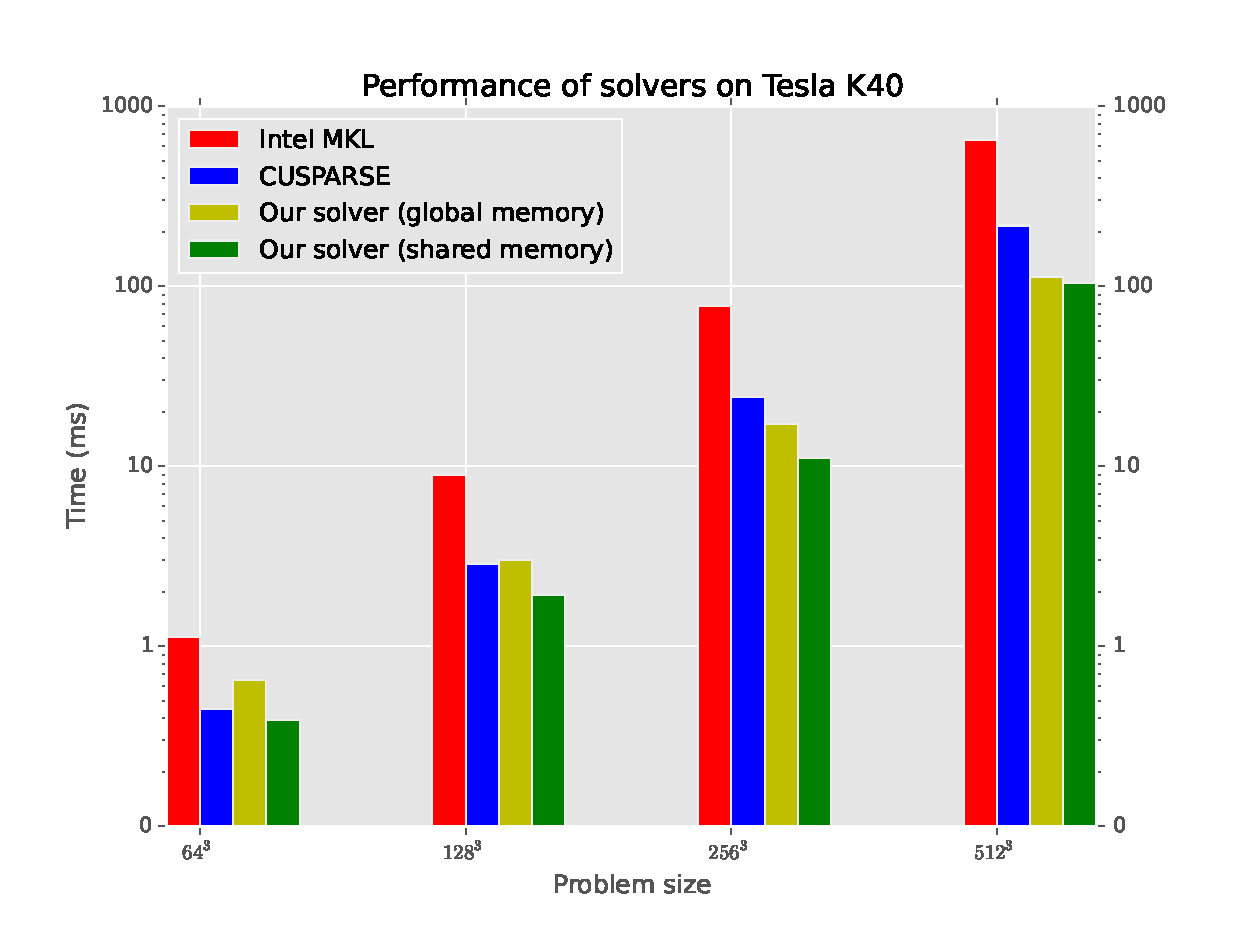
\includegraphics[height=200pt]{fig/compare-solvers-K40.eps}
\end{center}
\label{fig:compare-solvers-K40}
\end{figure}

\pagebreak
\section*{References}

\bibliography{references}
\bibliographystyle{elsarticle-num}
\end{document}
